\section{Benchmarks}
In this section we present some benchmarks\footnote{We have used the benchmark
library to this end \url{github.com/google/benchmark}.} 
performed to this new \boostfft\
library. Figure \ref{fig:benchmarks} show the mean values of the computation
time for our complex and real interfaces,
changing the \dft\ size, as we know that the size determines the underlying algorithm.
We then compare the results among the three available backends: \bsl, \gsl\ and \fftw.
The real types are the standard \verb|double| and the complex are represented as 
\verb|std::complex<double>|.
From that picture, we learn that our \bsl\ backend (blue lines) is in general two to three
orders of magnitude slower than the \gsl\ (in green) and \fftw\ (in red) libraries. 
The complexity of our algorithms, it can be appreciated, to scale as 
$\Order(N \log N)$ for any size $N$ (as claimed in section
\ref{sec:implementation}). The real \dft s take roughly half of the
computation time with respect to the complex transforms, see also table
\ref{tab:benchmarks}.
\begin{table}
    \centering
    \begin{tabular}{rrr}
        \dft\ size & $\Complex$ time (ms) & $\Real$ time (ms) \\
        \hline
4'096    &     2 &   1 \\
16'384   &    10 &   7 \\
65'536   &    53 &  37 \\
262'144  &   262 & 185 \\
1'048'576 &  1'238 & 891 \\
        \hline
100    & 2     & 1 \\
1'000   & 24    & 16 \\
10'000  & 311   & 205 \\
100'000 & 3'932  & 2'457 \\
1'000'000& 47'359 & 28'466 \\
        \hline
109     &    4  &    4  \\
1'009   &    56  &   56  \\
10'009  &   801  &  801  \\
100'003 &  10'107 &10'056  \\
    \end{tabular}
    \caption{Benchmarks for the \bsl\ backend, comparison of the real and
    complex \dft\ execution times. On top a series of powers of two sizes, in
    the middle a series of powers of ten sizes and in the bottom a series of
    prime sizes.}
    \label{tab:benchmarks}
\end{table}
\begin{figure}
    \centering
    \subfigure{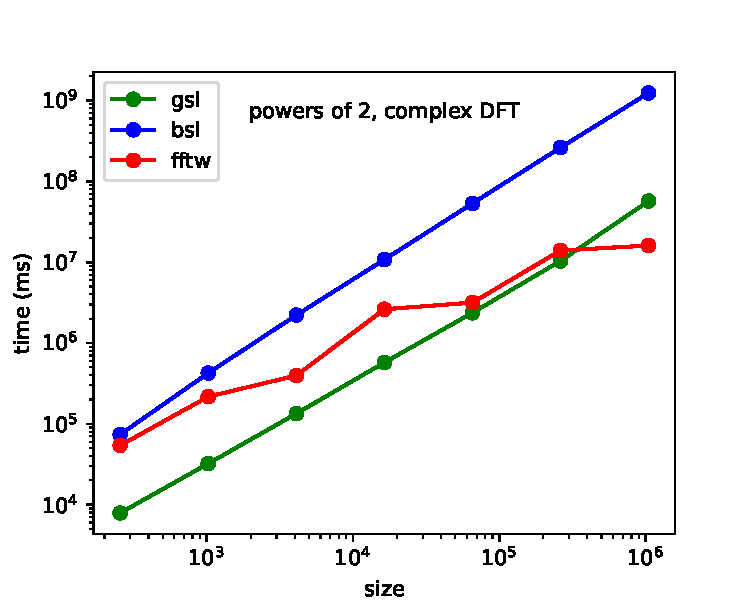
\includegraphics[width=0.49\textwidth]{plots/complex_p2.pdf}}
    \subfigure{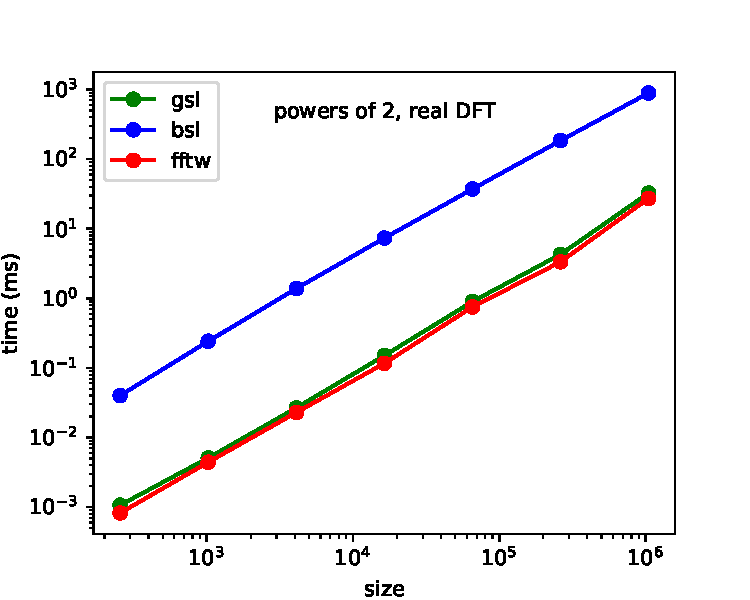
\includegraphics[width=0.49\textwidth]{plots/real_p2.pdf}}
    \vfill
    \subfigure{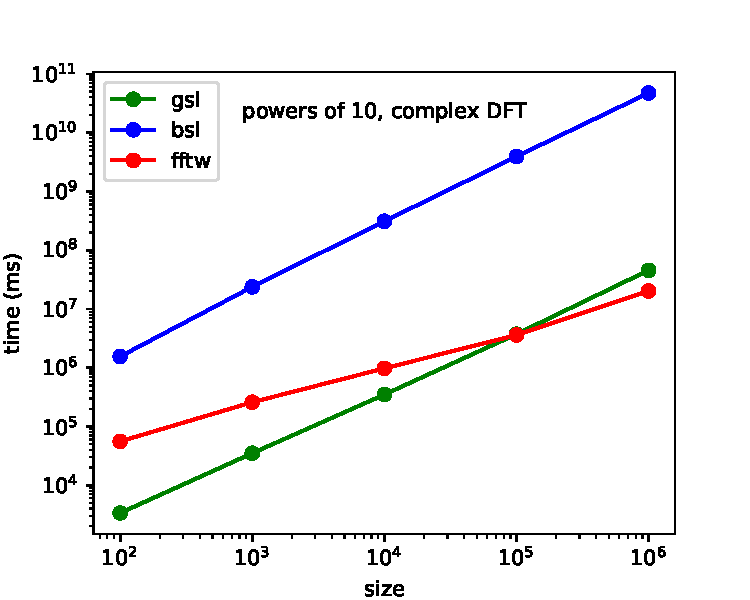
\includegraphics[width=0.49\textwidth]{plots/complex_p10.pdf}}
    \subfigure{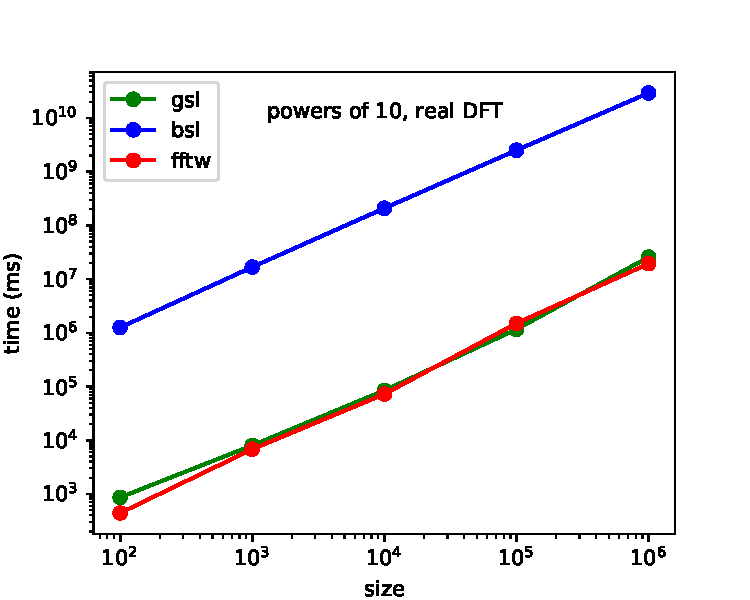
\includegraphics[width=0.49\textwidth]{plots/real_p10.pdf}}
    \vfill
    \subfigure{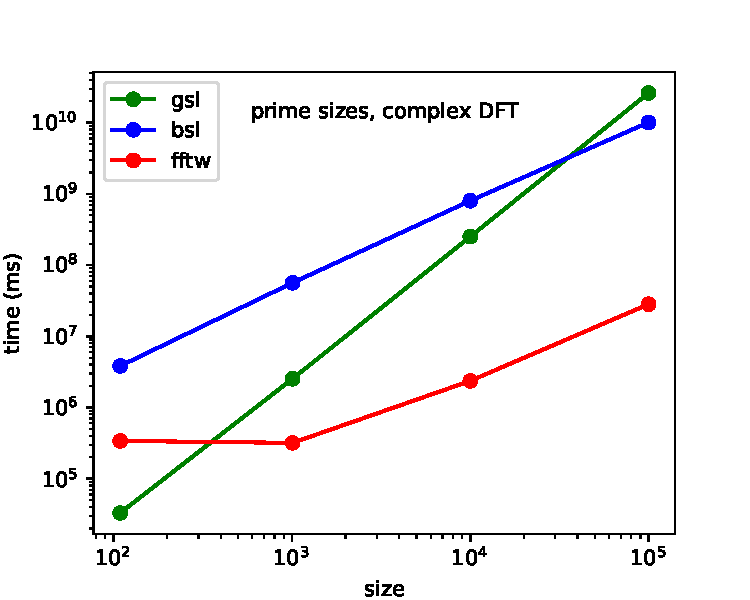
\includegraphics[width=0.49\textwidth]{plots/complex_primes.pdf}}
    \subfigure{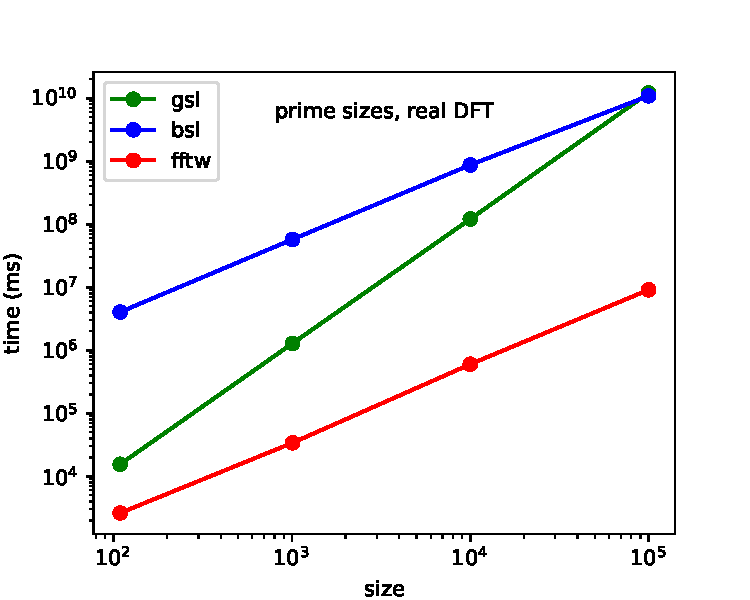
\includegraphics[width=0.49\textwidth]{plots/real_primes.pdf}}
    \caption{Benchmarks for different \dft\ sizes (rows), complex and real
    algorithms (columns), for our three backends: \bsl, \gsl\ and \fftw.}
    \label{fig:benchmarks}
\end{figure}


%\begin{figure}
%   \centering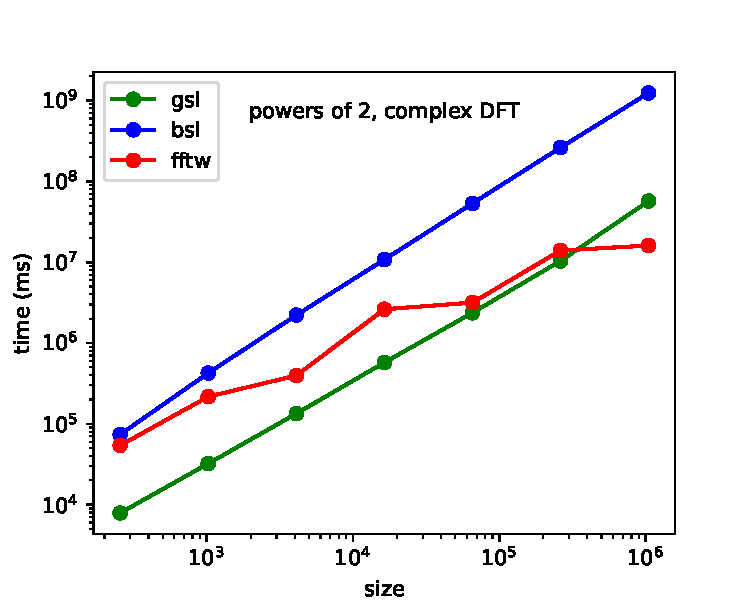
\includegraphics{plots/complex_p2.pdf} 
%   \caption{Benchmarks for powers of 2 sizes, double precision complex data.}
%\end{figure}
%\begin{figure}
%   \centering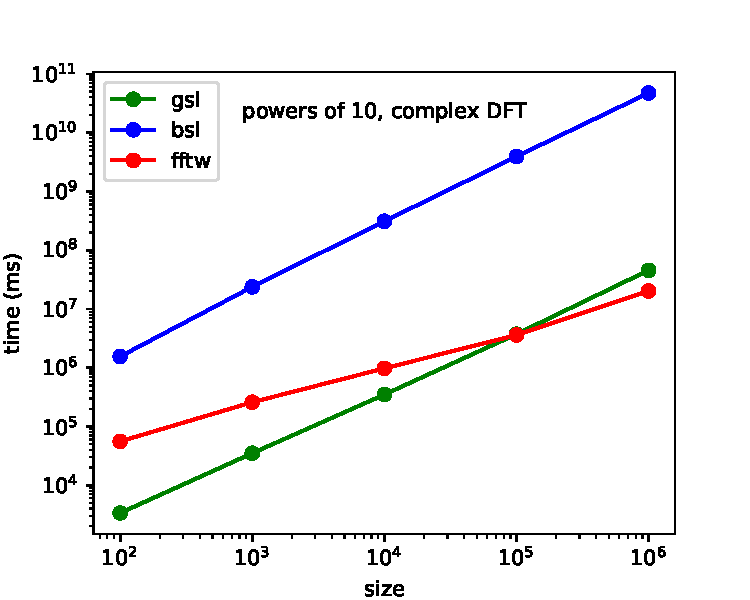
\includegraphics{plots/complex_p10.pdf} 
%   \caption{Benchmarks for powers of 10 sizes, double precision complex data.}
%\end{figure}
%\begin{figure}
%   \centering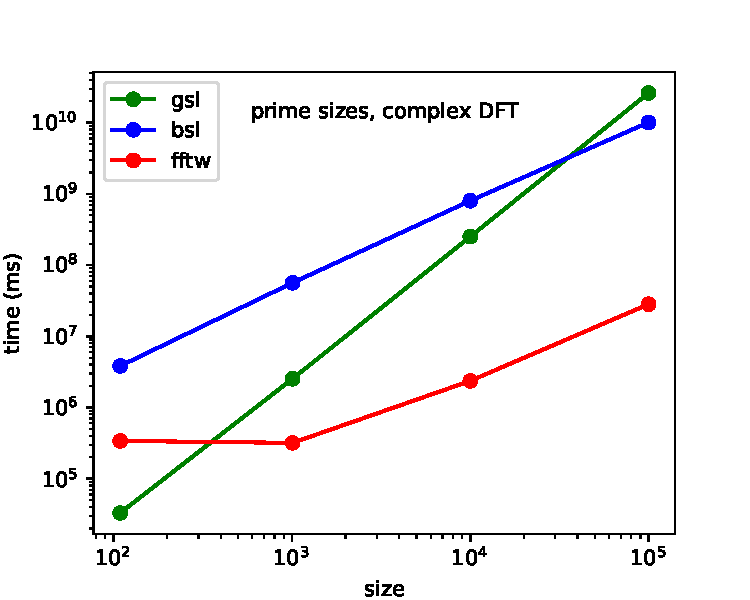
\includegraphics{plots/complex_primes.pdf} 
%   \caption{Benchmarks for prime sizes, double precision complex data.}
%\end{figure}
%
%\begin{figure}
%   \centering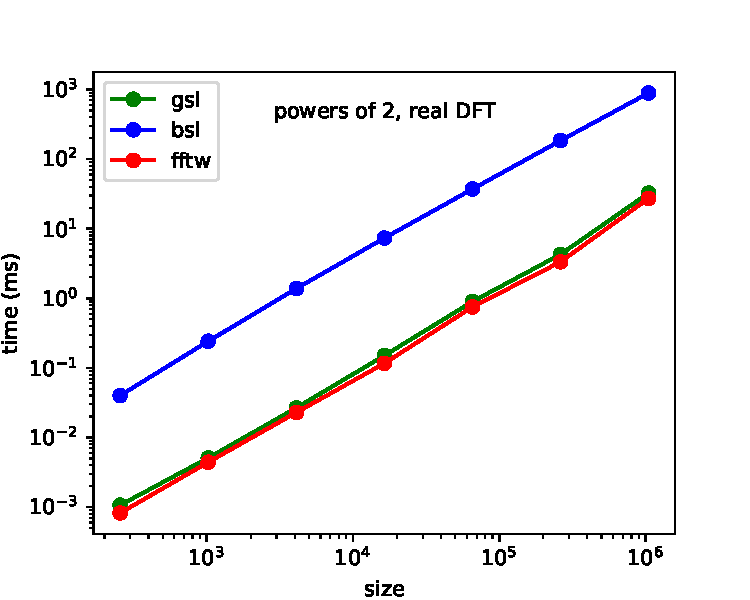
\includegraphics{plots/real_p2.pdf} 
%   \caption{Benchmarks for powers of 2 sizes, double precision real data.}
%\end{figure}
%\begin{figure}
%   \centering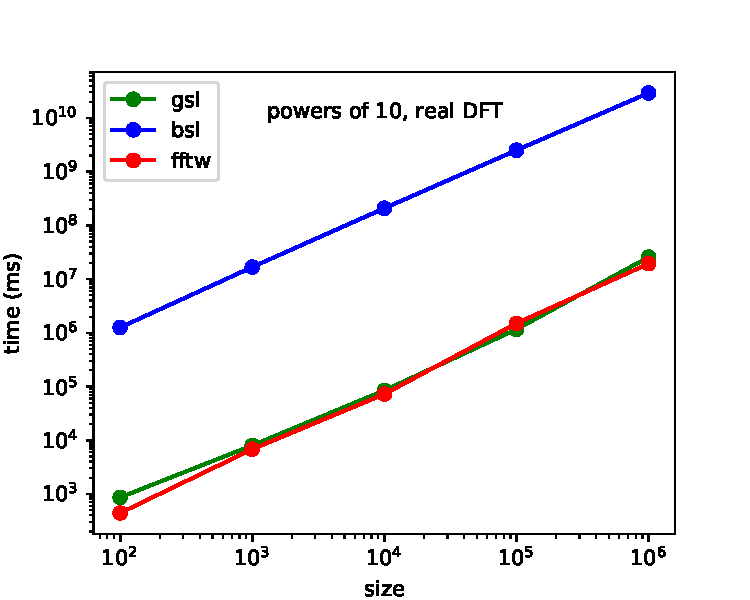
\includegraphics{plots/real_p10.pdf} 
%   \caption{Benchmarks for powers of 10 sizes, double precision real data.}
%\end{figure}
%\begin{figure}
%   \centering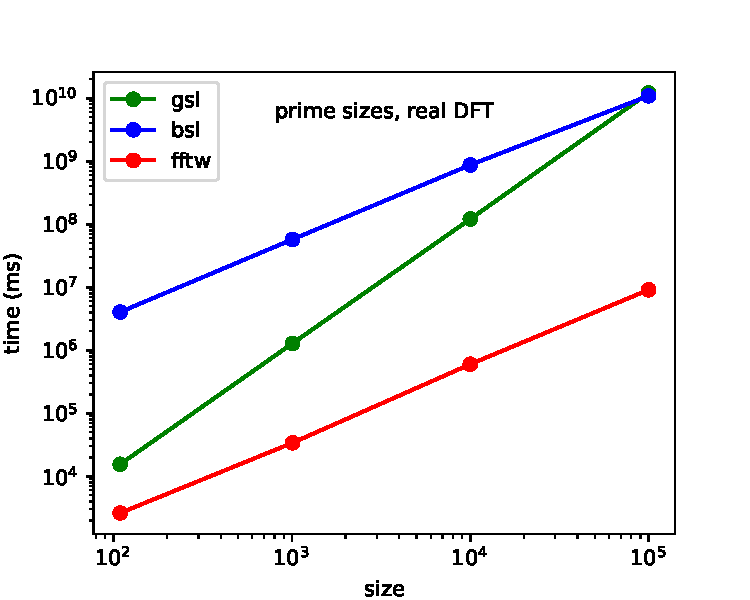
\includegraphics{plots/real_primes.pdf} 
%   \caption{Benchmarks for prime sizes, double precision real data.}
%\end{figure}
